    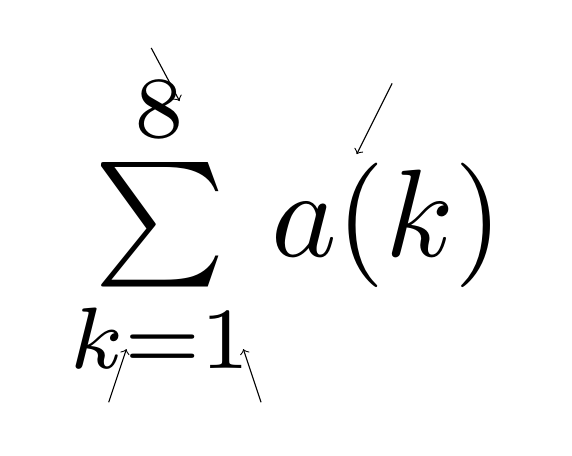
\begin{tikzpicture}[scale=4.5, every node/.style={transform shape}]
    \node at (0,0) {$\sum\limits_{k=1}^{8} a(k)$};
     \begin{scope}[every node/.style={scale=1}]
    \draw[->] (-0.5,-0.5) node[below] {\parbox{2cm}{}} --(-0.45,-0.35); %Laufindex/ \linebreak Laufvariable
    \draw[->] (-0.07,-0.5) node[below] {} --(-0.12,-0.35); %Startwert
    \draw[->] (-0.38,0.5) node[above] {} --(-0.3,0.35); %Endwert
    \draw[->] (0.3,0.4) node[above] {\parbox{2cm}{}} --(0.2,0.2); %Funktion bezgl. der Laufvariable
    \end{scope}
    \end{tikzpicture}